Consider one-dimensional nonlinear wave propagation in a spatially
heterogeneous medium, described by the first order hyperbolic system
\begin{subequations} \label{nel_pde}
\begin{align}
\epsilon_t(x,t)-u_x(x,t) & = 0 \\
\rho(x)u(x,t)_t - \sigma(\epsilon(x,t),x)_x & = 0.
\end{align}
\end{subequations}
%where the explicit spatial varation of the medium is periodic:
%\begin{align}
%\rho(x+\delta) & = \rho(x) & \sigma(\epsilon,x) & = \sigma(\epsilon,x+\delta).
%\end{align}
This system is a rather generic description of nonlinear waves in a 
Lagrangian frame, and arises in a variety
of contexts including elasticity, optics, and gas dynamics.
In the case of elasticity, $\epsilon,\sigma,\rho$, and $u$ are the
strain, stress, density, and velocity, respectively.

All the results presented in this work involve a simple periodic medium
composed of alternating homogeneous layers of materials A and B:
\begin{align} \label{LYmedium}
(\rho(x),K(x)) & = \left\{ \begin{array}{ll}
 (\rho_A,K_A) & \text{if } j< x < (j+1/2)
   \mbox{ for some integer j}, \\
 (\rho_B,K_B) & \mbox{otherwise.} \end{array}\right.
\end{align}
with nonlinear stress-strain relation
\be \label{expstress}
\sigma(\epsilon,x) = \exp(K(x)\epsilon) - 1,
\ee
Further computational experiments, to be reported elsewhere, suggest that 
the qualitative nature of our findings is typical for propagation in
more general periodic materials with quite general nonlinearities.


%\begin{align*}
%\epsilon(x,0) & = \exp(-(x-75)^2) & u(x,0) & = 0,
%\end{align*}
%The constitutive relation is taken to be
%\be \label{expstress}
%\sigma(\epsilon,x) = \exp(K(x)\epsilon) - 1,
%\ee
%although the qualitative results of these experiments do not seem
%to depend on the precise nature of this relation.

\subsection{Some suggestive numerical experiments}
To motivate the topic of this paper, we present the following simple experiments.
Consider the nonlinear wave equation
\eqref{nel_pde} with initial velocity zero and Gaussian initial stress, 
shown in Figure \ref{fig:ic}.
In the first experiment, we consider a homogeneous medium with $\rho(x)=K(x)=1$ 
and the solution is evolved for a short time. %to time $t=60$.  
As shown in Figure \ref{fig:experiment1_middle}, the initial 
hump evolves into a left-going
and a right-going pulse.  At the time shown, the sign of $u$ is negated,
and then the solution is evolved
again for the same length of time.  %to time $t=120$.  
The final solution is identical to the initial condition, as shown in Figure
\ref{fig:experiment1_end}.  The second half of the
experiment is, of course, identical to the first half, but in reverse.  
This follows from the fact that the equations are invariant under the
transformation $u \rightarrow -u$ and $t \rightarrow -t$.
%This demonstrates the time-reversibility of the solution.

\begin{figure}
\centerline{
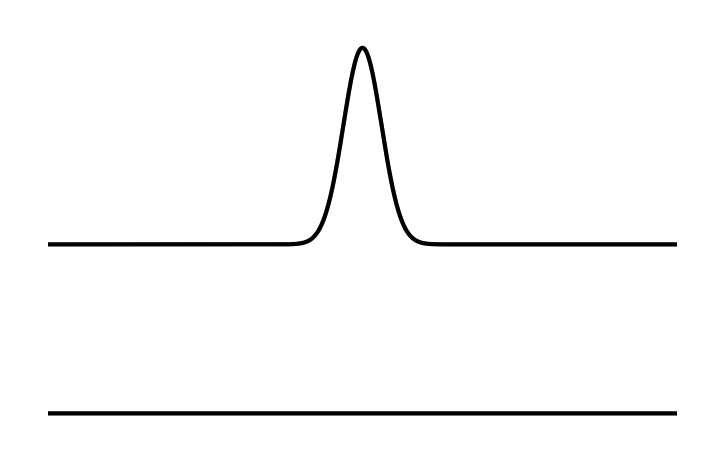
\includegraphics[width=2.5in]{figures/experiment1_ic.png}}
\caption{Initial condition for the three experiments.  In this and subsequent plots,
the upper plot is stress and the lower plot is velocity.\label{fig:ic}}
\end{figure}

\begin{figure}
\centerline{
\subfigure[Solution at $t=60$\label{fig:experiment1_middle}]{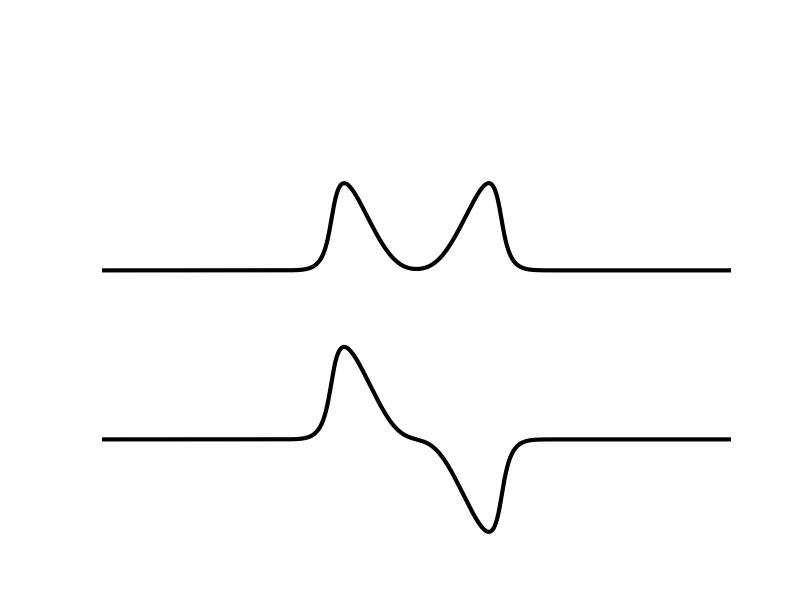
\includegraphics[width=3.0in]{figures/experiment1_middle.png}}
\subfigure[Solution at $t=120$\label{fig:experiment1_end}]{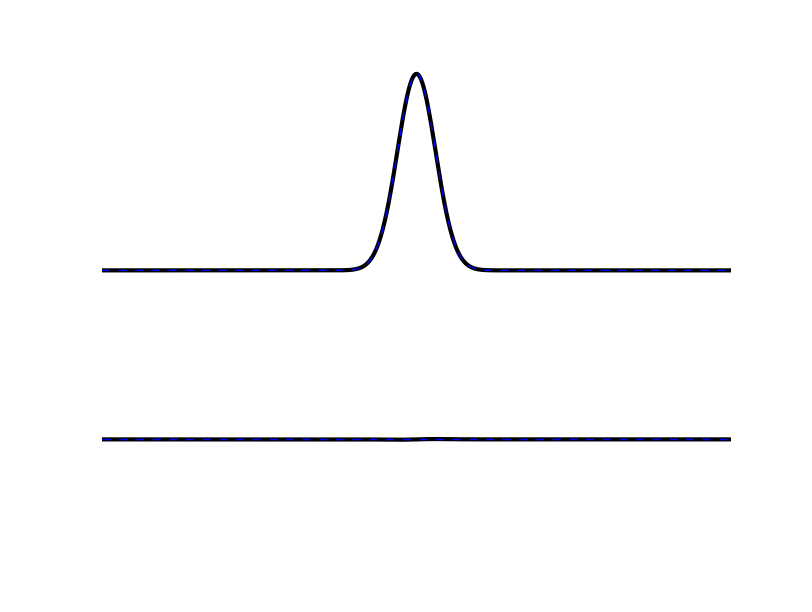
\includegraphics[width=3.0in]{figures/experiment1_end.png}}}
\caption{Stress (upper plot) and velocity (lower plot) snapshots of experiment 1, 
in which no shocks form.  The final
solution is identical to the initial condition.\label{fig:experiment1}}
\end{figure}

In the second experiment, again $\rho(x)=K(x)=1$ but now the solution is evolved
to a much later time.  % $t=250$.
As shown in Figure \ref{fig:experiment2_middle}, by this time the left- and 
right-going
pulses have developed shocks.  Again the velocity is reversed and the solution is
evolved for the same length of time.  %to time $t=500$.
In this case the final solution, shown in Figure \ref{fig:experiment2_end} 
is quite different from the initial condition.

\begin{figure}
\centerline{
\subfigure[Solution at $t=250$\label{fig:experiment2_middle}]{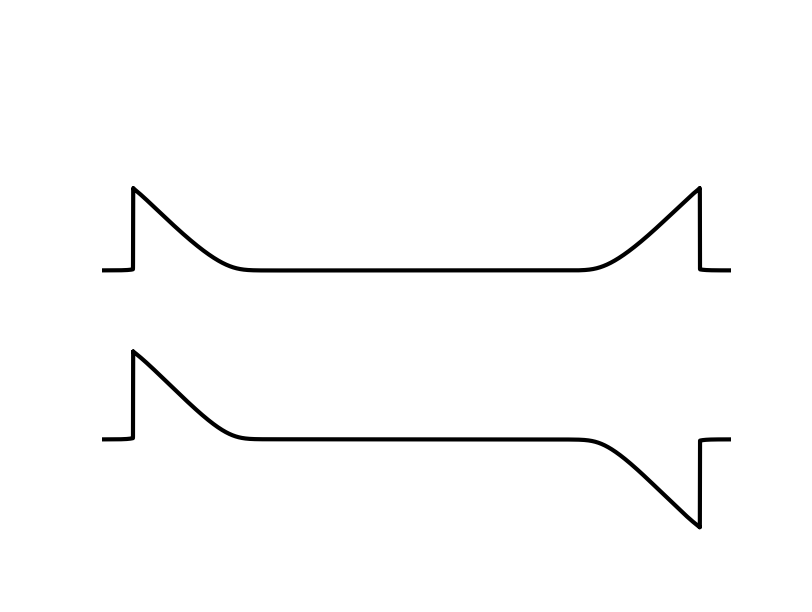
\includegraphics[width=3.0in]{figures/experiment2_middle.png}}
\subfigure[Solid line is solution at $t=500$; dotted line is initial condition\label{fig:experiment2_end}]{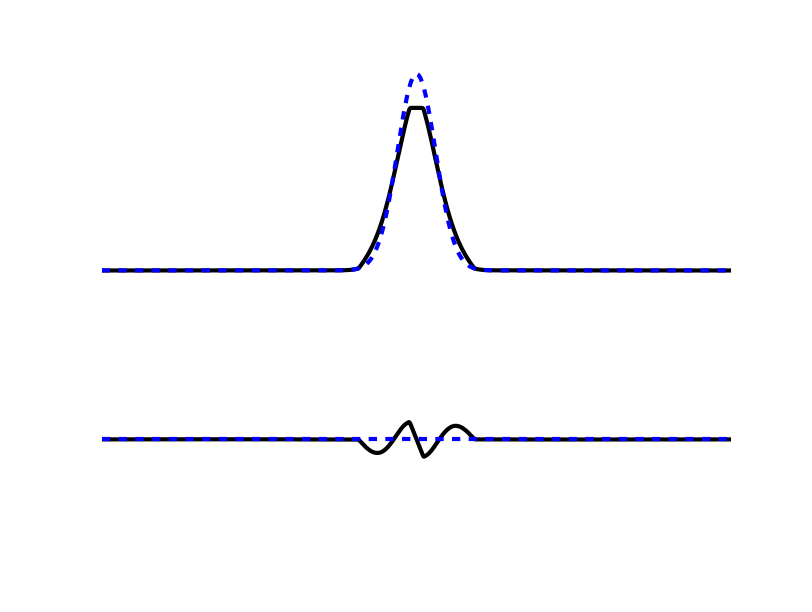
\includegraphics[width=3.0in]{figures/experiment2_end.png}}}
\caption{Stress and velocity snapshots of experiment 2, in which shocks form.\label{fig:experiment2}}
\end{figure}

In the third experiment, the medium is taken to be periodic and piecewise
constant, composed of alternating homogeneous layers of materials A and B,
as described by \eqref{LYmedium}, with $\rho_A=K_A=1$ and $\rho_B=K_B=4$.
The solution is evolved to the same time as in experiment two above. %$t=250$.
This time, highly oscillatory fronts develop, as shown in Figure \ref{fig:experiment3}.
Once again the velocity is reversed and 
the solution evolved for the same length of time. % $t=500$.  
In this case the final solution appears identical to the initial condition.

\begin{figure}
\centerline{
\subfigure[Solution at $t=250$]{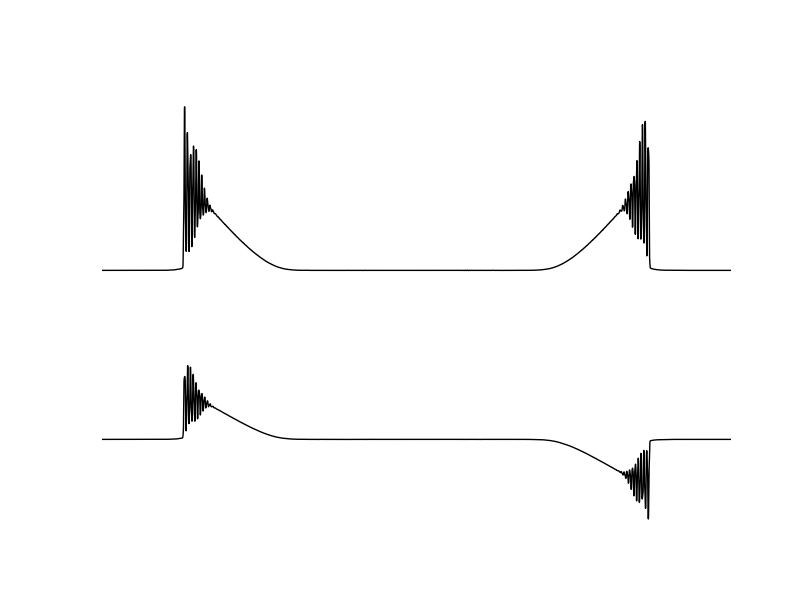
\includegraphics[width=3.0in]{figures/experiment3_middle.png}}
\subfigure[Solution at $t=500$]{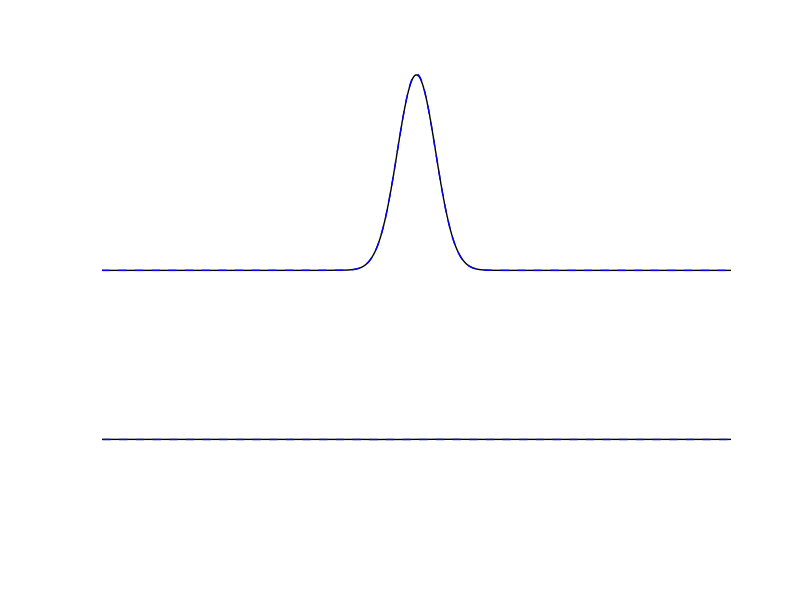
\includegraphics[width=3.0in]{figures/experiment3_end.png}}}
\caption{Stress and velocity snapshots of experiment 3, in a periodic medium.  The final solution is identical to the initial condition.\label{fig:experiment3}}
\end{figure}

\subsection{First-order hyperbolic systems theory}
The results of the first two experiments are well understood within the existing
mathematical theory of hyperbolic conservation laws.  The system \eqref{nel_pde}
is time-reversible as long as the solution remains smooth.
In the first experiment, since shocks do not form,
the solution satisfies the nonlinear wave equation \eqref{nel_pde} 
in a strong sense and is time-reversible.
In the second experiment, characteristics meet and shocks form, leading to
a loss of information.  In fact, whereas the initial condition we have used
is the only one
that leads to the solution shown in Figure \ref{fig:experiment1_middle}
at the given time, there are infinitely many initial conditions that lead
to the solution shown in Figure \ref{fig:experiment2_middle}; the 
curves in Figure \ref{fig:experiment2_end} are two of them.
In general, such irreversible behavior is
expected whenever the solution is evolved past the time of shock formation.
Thus, from the point of view of the classical theory for nonlinear hyperbolic
systems, the long-time reversibility of waves in the periodic
medium observed in the third experiment seems remarkable.
%since solutions of 
%the nonlinear elasticity equations \eqref{nel_pde} with uniform coefficients
%generically develop discontinuities after a short time; indeed, this
%is typical of solutions to nonlinear first-order hyperbolic 
%systems in general (see, e.g. \cite{levequefvmbook}).
Similar waves in a homogeneous medium composed of material A
or material B would not be reversible at this late time. 

%In most applications, the appropriate definition of weak solution
%for a first-order hyperbolic system is understood in terms of a
%vanishing-viscosity limit, and numerical methods are designed 
%to converge to such weak solutions.  We take this point of view
%also in our work.

\subsection{Dispersive nonlinear wave theory}
It was shown in \cite{santosa1991} that for linear waves whose wavelength is
long relative to the period of the medium, the leading order
effect of material periodicity is an effective dispersion.
Correspondingly, dispersive wave equations are often introduced to model
the effect of periodic microstructure \cite{Rubin2009}.
Indeed, a system of dispersive effective equations for the elasticity system
\eqref{nel_pde} with periodic coefficients was derived in \cite{leveque2003} 
and shown to agree with results from direct simulation.
Dispersive nonlinear wave equations lead to the appearance of so-called
{\em dispersive shock waves}, consisting of a high-amplitude oscillatory
front followed by a more slowly varying tail \cite{El2005}.
The waves in \Fig{experiment3} strongly resemble these dispersive shocks.
In such systems, the dispersive term(s) in the equation
can often be shown to regularize the solution, preventing the appearance of 
discontinuities.  Hence time-reversibility is typically a property of such
dispersive nonlinear systems.

However, the effective dispersive equations of \cite{leveque2003}, like
many dispersive continuum models, rely on an assumption that the wavelength of
the solution is large relative to the period of the medium.  Since nonlinearity
leads to the appearance of high frequencies in the solution, it seems at
least possible that this model will break down.  One may ask, then,
whether true shocks (discontinuities) may indeed appear.

The answer to this question turns out to be quite interesting.  As suggested
already by the third experiment above,
it appears that shocks do not form, even after very long times
so long as the amplitude of the initial conditions is not too large 
relative to the effective dispersion induced by material periodicity.
Furthermore, initial shocks with small amplitude appear to be unstable
and vanish after a short time.
For larger-amplitude solutions, (or weaker effective material dispersion) 
shock discontinuities appear and persist.
Empirically, we find an approximate condition discriminating between data 
that will or will not lead to shocks, in the form of a characteristic condition 
that can be seen as a 
generalization of the well-known Lax entropy condition for shock admissibility.

In the remainder of this section, we describe briefly the numerical
methods used in this work.  In Section \ref{measures},
we discuss the problem of detecting shock formation and propose two
robust computational approaches.  Along the way, we make some 
observations about limiters used in high-resolution shock-capturing methods.  In Section 
\ref{criterion}, we hypothesize
a condition for shock formation in solutions of the nonlinear wave equation
\eqref{nel_pde} in the presence of a periodic medium and
conduct some further numerical tests for layered media that support the
proposed condition.  In Section \ref{discussion}, 
we discuss the significance of the results and possible generalizations.

The results presented here can be understood even better when accompanied
by animations of the wave behavior described.  These are available online,
along with all code for reproducing the computational results described,
at \url{http://bitbucket.org/ketch/layeredmediashocks/src}.
The reader is highly encouraged to view the animations and experiment
with the simulations.

\subsection{Numerical discretization\label{discretization}}
Before continuing, we briefly describe the numerical methods used for the
computations presented in this work.  The methods employed are both
finite volume Godunov-type
high-resolution methods, which employ Riemann solvers and nonlinear limiters
to obtain good resolution of shocks or steep gradients without spurious
oscillations.  

The first method used is that implemented in Clawpack \cite{clawpack45}
and described in \cite{leveque1997}.  Briefly, this is a second-order TVD
high-resolution scheme based on Lax-Wendroff discretization with limiters.

The second method used is that implemented in the SharpClaw software package
\cite{sharpclaw} and described in \cite{ketcheson2006,ketcheson2011}.  
This involves a method-of-lines
discretization approach, using WENO reconstruction in space and high order
Runge-Kutta time integration.  In all experiments with SharpClaw we use the
fourth-order SSP Runge-Kutta scheme of \cite{ketcheson2008} and fifth-order 
WENO reconstruction.


%This experiment suggests many interesting questions. In the present work
%we attempt to answer two of them through further computational experiments and
%analysis.
%First, the results seem to indicate that shocks have not formed in the 
%periodic medium, even after long times.
%%formation has occurred, although a closer look indicates that it has not.
%%whereas the time-reversibility indicates that it has not.  
%% RJL: this original sentence didn't make so much sense because
%% time-reversibility only holds until shocks form.

%Hence our first question:
%
%\begin{quotation}
%{\bf Q1:} {\em Can a nonlinear first-order hyperbolic system with convex flux
%possess non-monotone solutions that are continuous for all time if 
%the coefficients are allowed to vary in space?}
%\end{quotation}
%
%We attempt to justify an affirmative answer to
%this question through further experiments.
%We will also see that this effect 
%depends critically on the impedance variation in the medium, and that
%there exists a dramatic phase transition with respect to shock formation
%as the impedance mismatch varies.
%Our second question is thus:
%
%\begin{quotation}
%{\bf Q2:} {\em What properties of the material and/or initial conditions 
%determine whether shocks will form?}
%\end{quotation}
%



%\section{Solitary waves in periodic media}
%{\bf Remove this section?}
%%It was shown in \cite{santosa1991} that for linear waves whose wavelength is
%%long relative to the period of the medium, the leading order
%%effect of material periodicity is an effective dispersion.
%%In LeVeque \cite{leveque2002} and LeVeque \& Yong \cite{leveque2003},
%%simulations of a one-dimensional layered nonlinear elastic 
%%medium gave rise to solitary waves, apparently due to
%%the combined effects of nonlinearity and the aforementioned effective dispersion.  
%
%The third experiment above (pictured in Figure \ref{fig:experiment3})
%was motivated by computational experiments performed
%in \cite{leveque2003}, which we briefly review here.
%The stress relation is taken as \eqref{expstress}, and the medium is
%defined by \eqref{LYmedium} with
%$$\rho_A=K_A=1, \mbox{  and  } \rho_B=K_B=4.$$
%An initial pulse is generated by motion of the left boundary:
%\begin{align*}
%u(0,t) & = \begin{cases} 
%  -0.1(1+\cos(\pi(t-10)/10)) & \mbox{for } 0\le t\le 20 \\
%  0 & \mbox{for } t>20. \end{cases}
%\end{align*}
%After a short time, periodic boundary conditions are imposed in
%order to observe the long-time behavior of the pulse without using
%an excessively large computational domain.
%The initial half-cosine pulse evolves into a train
%of solitary waves, as shown in Figure \ref{fig:stego}.
%Because of the discontinuous appearance of strain profiles
%(see Figure \ref{fig:strain_train})
%of the solitary waves, they were dubbed 'stegotons'.  In \cite{leveque2003},
%they were shown to
%have many soliton-like properties; for instance, solitary waves of 
%differing amplitude have nearly the same shape when properly rescaled,
%and stegoton interactions appear to result in only a phase shift.
%The waves were related to the Toda lattice and were also analyzed using
%homogenized equations.
%
%These waves have recently been further investigated both experimentally and
%computationally in \cite{berezovski2006}.  The stegoton problem was also
%used in \cite{xu2007} as a verification test for a method of handling
%material discontinuities.  On-going experiments indicate that solitary waves
%arise fairly generally in the solution of the nonlinear wave equation
%\eqref{nel_pde}, for different nonlinearities and different kinds of
%periodic media.  
%
%%Further investigation in this vein is ongoing, but
%%to suggest the broad applicability of our results, we will consider 
%%two kinds of media in this work.  The first is the medium given by
%%\eqref{LYmedium}.  The second is a smoothly varying medium:
%%\begin{subequations}
%%\label{eq:sinmat}
%%\begin{align}
%%\rho(x) = & a + b \sin\left(2\pi \frac{x}{\delta}\right) \\
%%K(x) = & a + b \sin\left(2\pi\left(\frac{x}{\delta}+\theta\right)\right)
%%\end{align}
%%\end{subequations}
%
%
%\begin{figure}
%\subfigure[Initial pulse]{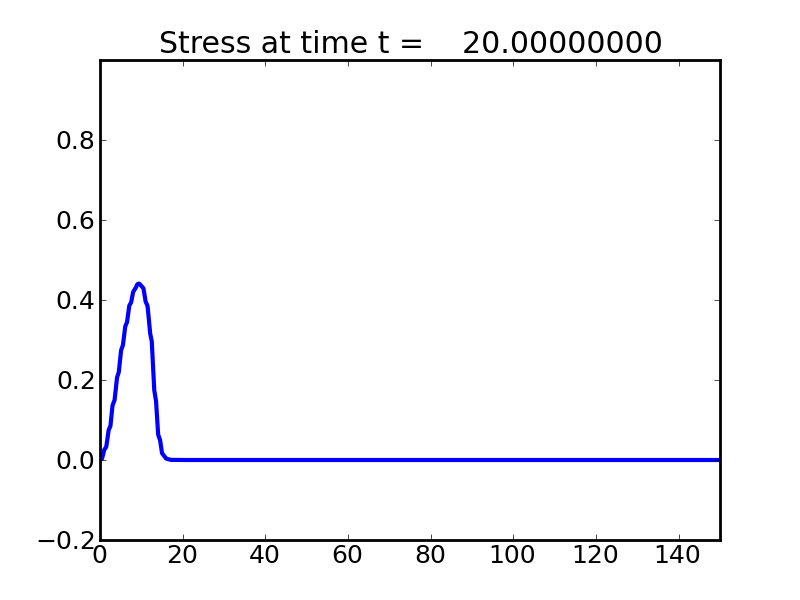
\includegraphics[width=2.5in]{figures/intro_initial_pulse.png}}
%\subfigure[Pulse steepens due to nonlinearity]{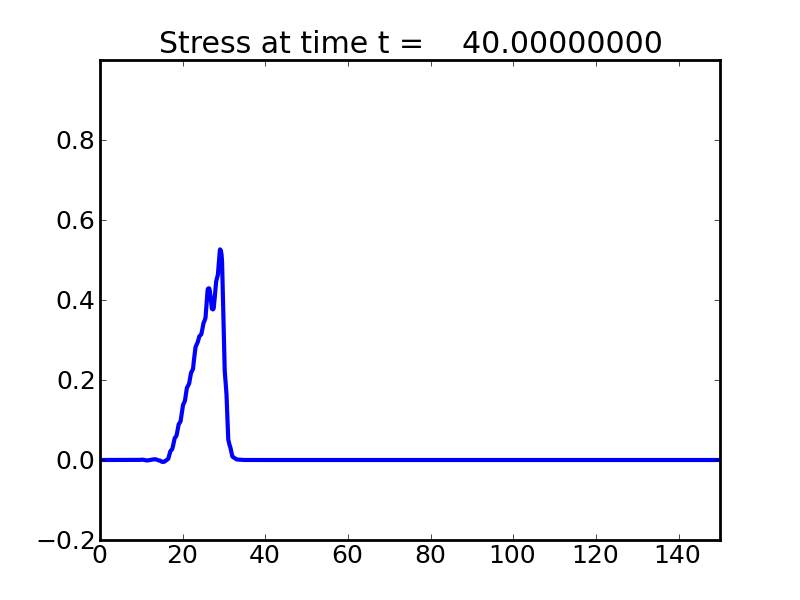
\includegraphics[width=2.5in]{figures/intro_steepens.png}}
%\subfigure[Separation into solitary waves]{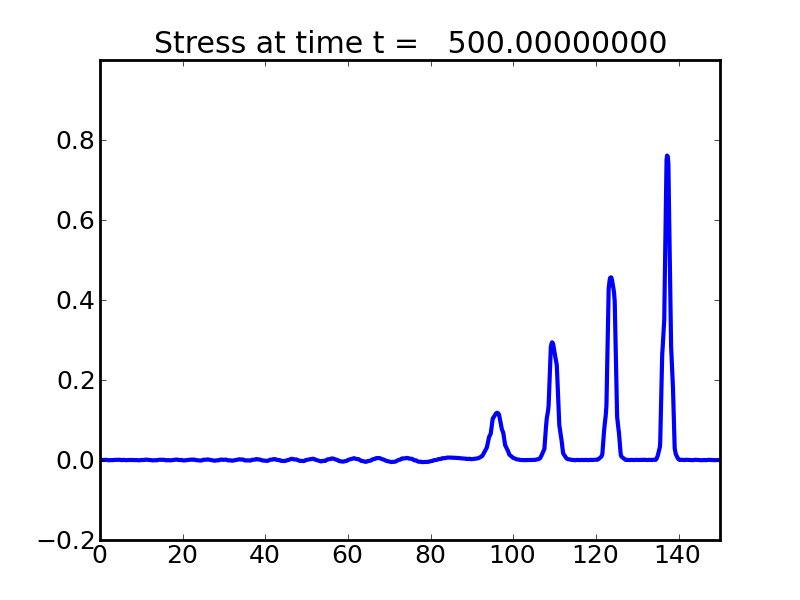
\includegraphics[width=2.5in]{figures/intro_stegotons.png}}
%\subfigure[Closeup of leading pulse]{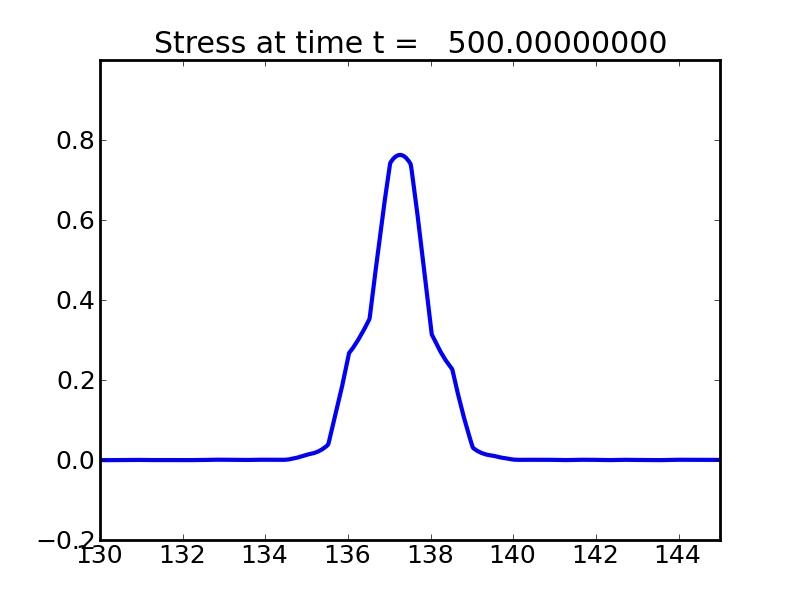
\includegraphics[width=2.5in]{figures/intro_closeup.png}}
%\caption{Evolution of a single pulse into a solitary wave train. \label{fig:stego}}
%\end{figure}
%
%\begin{figure}
%\centerline{
%\includegraphics[width=6in]{figures/stegotons_strain.eps}}
%\caption{Strain profile of solitary wave train.\label{fig:strain_train}}
%\end{figure}
%
%
%%The second question of interest in this work addresses the generality
%%of this phenomenon.  
%%
%%{\bf What characteristics of a periodic non-dispersive medium lead
%%to the production of solitary waves?}
